\documentclass[12pt,a4paper]{article}

\usepackage[T2A]{fontenc}
\usepackage[utf8]{inputenc}
\usepackage[english,russian]{babel}
\usepackage{geometry}
\usepackage{graphicx}
\usepackage{float}
\usepackage{caption}
\usepackage{array}
\usepackage{booktabs}
\usepackage{longtable}
\usepackage{tabularx}
\usepackage{enumitem}
\usepackage{tikz}
\usepackage{xcolor}
\usepackage{hyperref}
\usepackage{fancyhdr}

\usetikzlibrary{arrows.meta,positioning,shapes.geometric}

\geometry{
  left=2.5cm,
  right=1.5cm,
  top=2cm,
  bottom=2cm
}

\hypersetup{
  colorlinks=true,
  linkcolor=black,
  urlcolor=blue,
  pdftitle={Отчёт по лабораторной работе №1},
  pdfauthor={Цыканов Артём Эдуардович}
}

\graphicspath{{docs/screenshots/}}
\setlength{\parindent}{1.25cm}
\setlength{\parskip}{0.25em}
\setlist{nosep}
\captionsetup{font=small,labelfont=bf}

\pagestyle{fancy}
\fancyhf{}
\fancyhead[L]{Лабораторная работа №1}
\fancyhead[R]{Проектирование AI-сервиса на FastAPI}
\fancyfoot[C]{\thepage}
\setlength{\headheight}{15pt}

\newcolumntype{Y}{>{\raggedright\arraybackslash}X}
\newcommand{\code}[1]{\texttt{#1}}

\begin{document}

\begin{titlepage}
  \begin{center}
    \textbf{МИНИСТЕРСТВО НАУКИ И ВЫСШЕГО ОБРАЗОВАНИЯ\\
    РОССИЙСКОЙ ФЕДЕРАЦИИ}

    \vspace{0.5cm}

    Федеральное государственное автономное образовательное учреждение\\
    высшего образования

    \vspace{0.3cm}

    \textbf{«НАЦИОНАЛЬНЫЙ ИССЛЕДОВАТЕЛЬСКИЙ\\
    ТЕХНОЛОГИЧЕСКИЙ УНИВЕРСИТЕТ «МИСИС»»}

    \vspace{1.5cm}

    \textbf{Институт компьютерных наук}\\[0.3cm]
    \textbf{Кафедра инженерной кибернетики}

    \vspace{1.7cm}

    \textbf{ЛАБОРАТОРНАЯ РАБОТА №1}\\[0.4cm]
    по дисциплине «Современные интеллектуальные сетевые сервисы»

    \vspace{1.5cm}

    {\Large\bfseries Проектирование AI-сервиса на FastAPI}
  \end{center}

  \vfill

  \begin{flushright}
    \begin{tabular}{@{}ll@{}}
      Выполнил: & студент группы МПИ-25-1-1 \\
                & Цыканов Артём Эдуардович \\[0.5cm]
      Проверил: & И.~О. Фамилия \\
    \end{tabular}
  \end{flushright}

  \vfill

  \begin{center}
    Москва, 2026
  \end{center}
\end{titlepage}

\tableofcontents
\newpage

\section{Цель работы}

Изучить принципы проектирования REST API для AI-сервиса, реализовать контур
инференса на FastAPI, описать контракт при помощи Pydantic и OpenAPI, а также
проверить корректную обработку запросов и ошибок.

\section{Архитектура сервиса}

Сервис работает синхронно: клиент отправляет данные в формате JSON и получает
оценку риска в рамках одного HTTP-запроса. Pydantic проверяет структуру данных,
сервисный слой контролирует бизнес-ограничения, условная ML-модель рассчитывает
числовую оценку риска, а постобработка формирует категорию и рекомендацию.
Полученный результат сохраняется в оперативной памяти.

\begin{figure}[H]
  \centering
  \resizebox{\textwidth}{!}{%
    \begin{tikzpicture}[
      node distance=9mm,
      block/.style={draw, rounded corners, align=center, minimum height=11mm,
                    minimum width=25mm, fill=blue!6},
      storage/.style={draw, cylinder, shape border rotate=90, aspect=0.25,
                     align=center, minimum height=14mm, minimum width=22mm,
                     fill=green!8},
      arrow/.style={-{Latex[length=2.5mm]}, thick}
    ]
      \node[block] (client) {Клиент\\CRM / Web / Mobile};
      \node[block, right=of client] (api) {FastAPI\\HTTP-слой};
      \node[block, right=of api] (validation) {Pydantic-\\валидация};
      \node[block, right=of validation] (business) {Бизнес-\\валидация};
      \node[block, right=of business] (model) {Расчёт\\риска};
      \node[block, right=of model] (post) {Постобработка};
      \node[storage, right=of post] (storage) {In-memory\\storage};

      \draw[arrow] (client) -- node[above, font=\small]{HTTP/JSON} (api);
      \draw[arrow] (api) -- (validation);
      \draw[arrow] (validation) -- (business);
      \draw[arrow] (business) -- (model);
      \draw[arrow] (model) -- (post);
      \draw[arrow] (post) -- (storage);
      \draw[arrow, bend right=35] (post.south) to
        node[below, font=\small]{PredictionResponse} (api.south);
    \end{tikzpicture}%
  }
  \caption{Компонентная схема сервиса агроскоринга}
  \label{fig:architecture}
\end{figure}

Приложение разделено на следующие программные компоненты:

\begin{itemize}
  \item \code{main.py} --- HTTP-слой, middleware и маршруты FastAPI;
  \item \code{schemas.py} --- Pydantic-схемы запросов и ответов;
  \item \code{model.py} --- функция расчёта риска;
  \item \code{services.py} --- бизнес-валидация и постобработка;
  \item \code{storage.py} --- временное in-memory хранилище прогнозов.
\end{itemize}

Исходный код решения размещён в каталоге \href{run:./}{\code{lab\_01}}
репозитория решений.

\section{Реализованные endpoints}

\begin{table}[H]
  \centering
  \caption{Endpoints сервиса}
  \label{tab:endpoints}
  \begin{tabularx}{\textwidth}{>{\ttfamily}p{4.3cm} p{1.5cm} Y}
    \toprule
    \normalfont\textbf{Endpoint} & \textbf{Метод} & \textbf{Назначение} \\
    \midrule
    /health & GET & Проверка работоспособности HTTP API \\
    /model-info & GET & Получение метаданных и статуса готовности модели \\
    /predict & POST & Валидация, инференс и сохранение прогноза \\
    /predictions/\{request\_id\} & GET & Поиск сохранённого прогноза по UUID \\
    /predictions & GET & Список прогнозов с фильтром и ограничением количества \\
    \bottomrule
  \end{tabularx}
\end{table}

Endpoint \code{POST /predict} возвращает \code{200 OK}, поскольку его основная
семантика --- синхронное вычисление результата. Внутреннее сохранение прогноза
не делает этот endpoint классической операцией создания ресурса со статусом
\code{201 Created}.

Endpoint \code{/health} проверяет доступность самого HTTP API, а
\code{/model-info} сообщает сведения о конкретной модели и её готовности.
Поэтому API может оставаться доступным, когда модель временно не готова к
инференсу.

\section{Документация и проверка через Swagger UI}

FastAPI автоматически сформировал OpenAPI-описание сервиса и интерактивную
документацию Swagger UI. В документации представлены все пять маршрутов,
Pydantic-схемы, ограничения параметров и возможные HTTP-коды.

\begin{figure}[H]
  \centering
  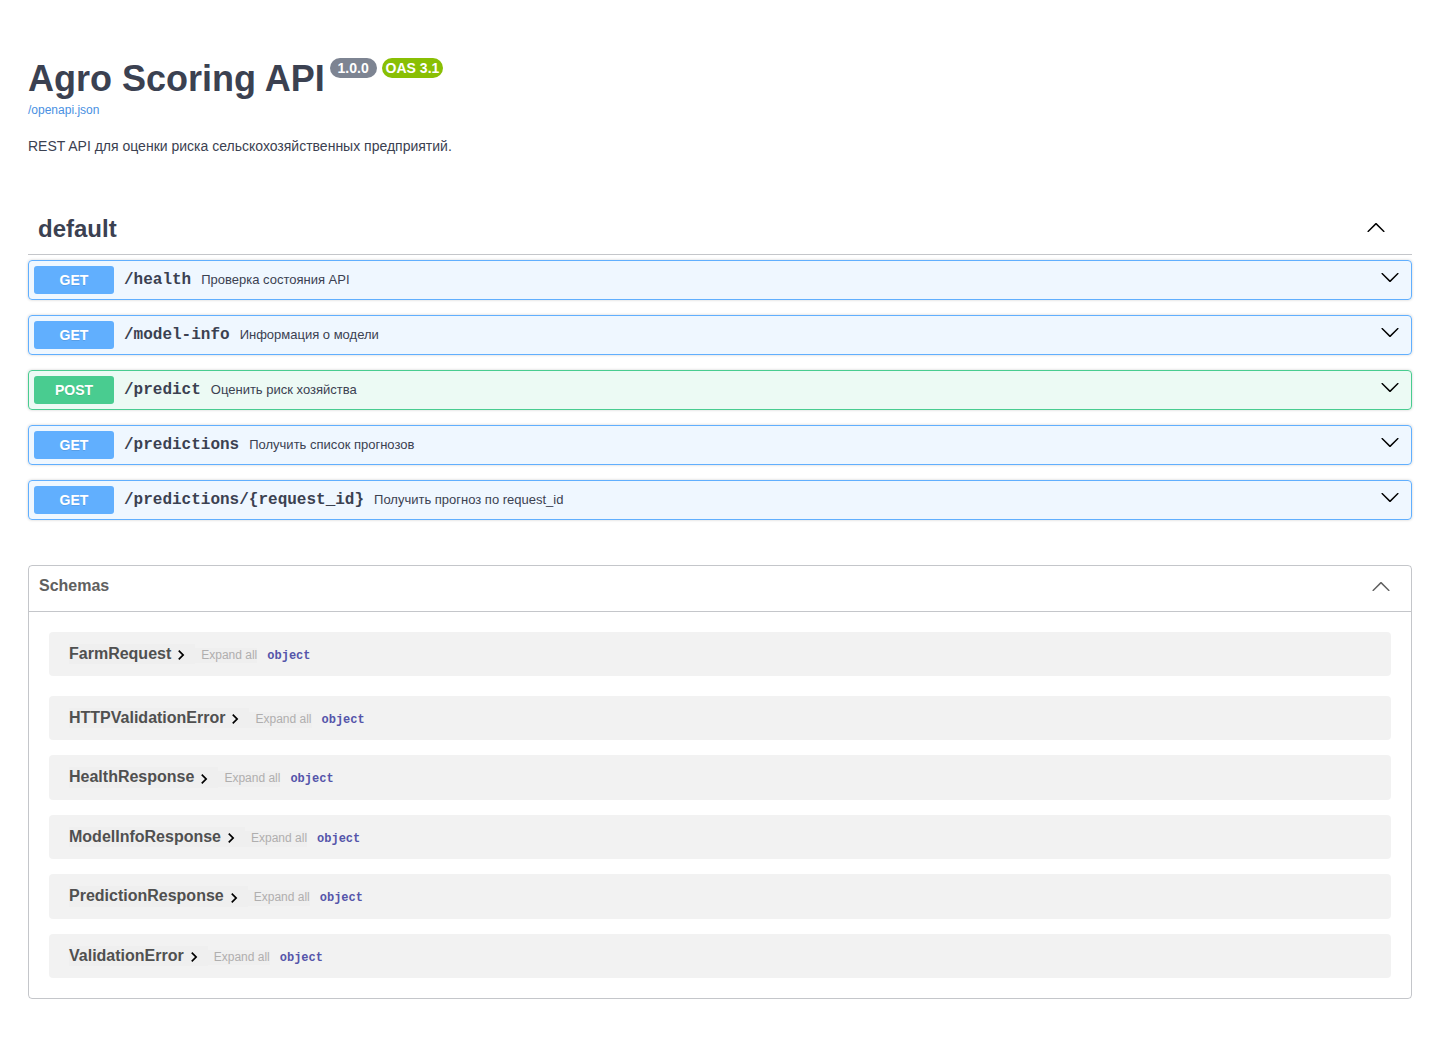
\includegraphics[width=\textwidth,height=0.78\textheight,keepaspectratio]{swagger-ui.png}
  \caption{Общий вид Swagger UI}
  \label{fig:swagger}
\end{figure}

\subsection{Успешное выполнение прогноза}

Для корректного запроса сервис рассчитал оценку риска \code{0.9}, присвоил
категорию \code{high}, сформировал рекомендацию и вернул ответ со статусом 200.

\begin{figure}[H]
  \centering
  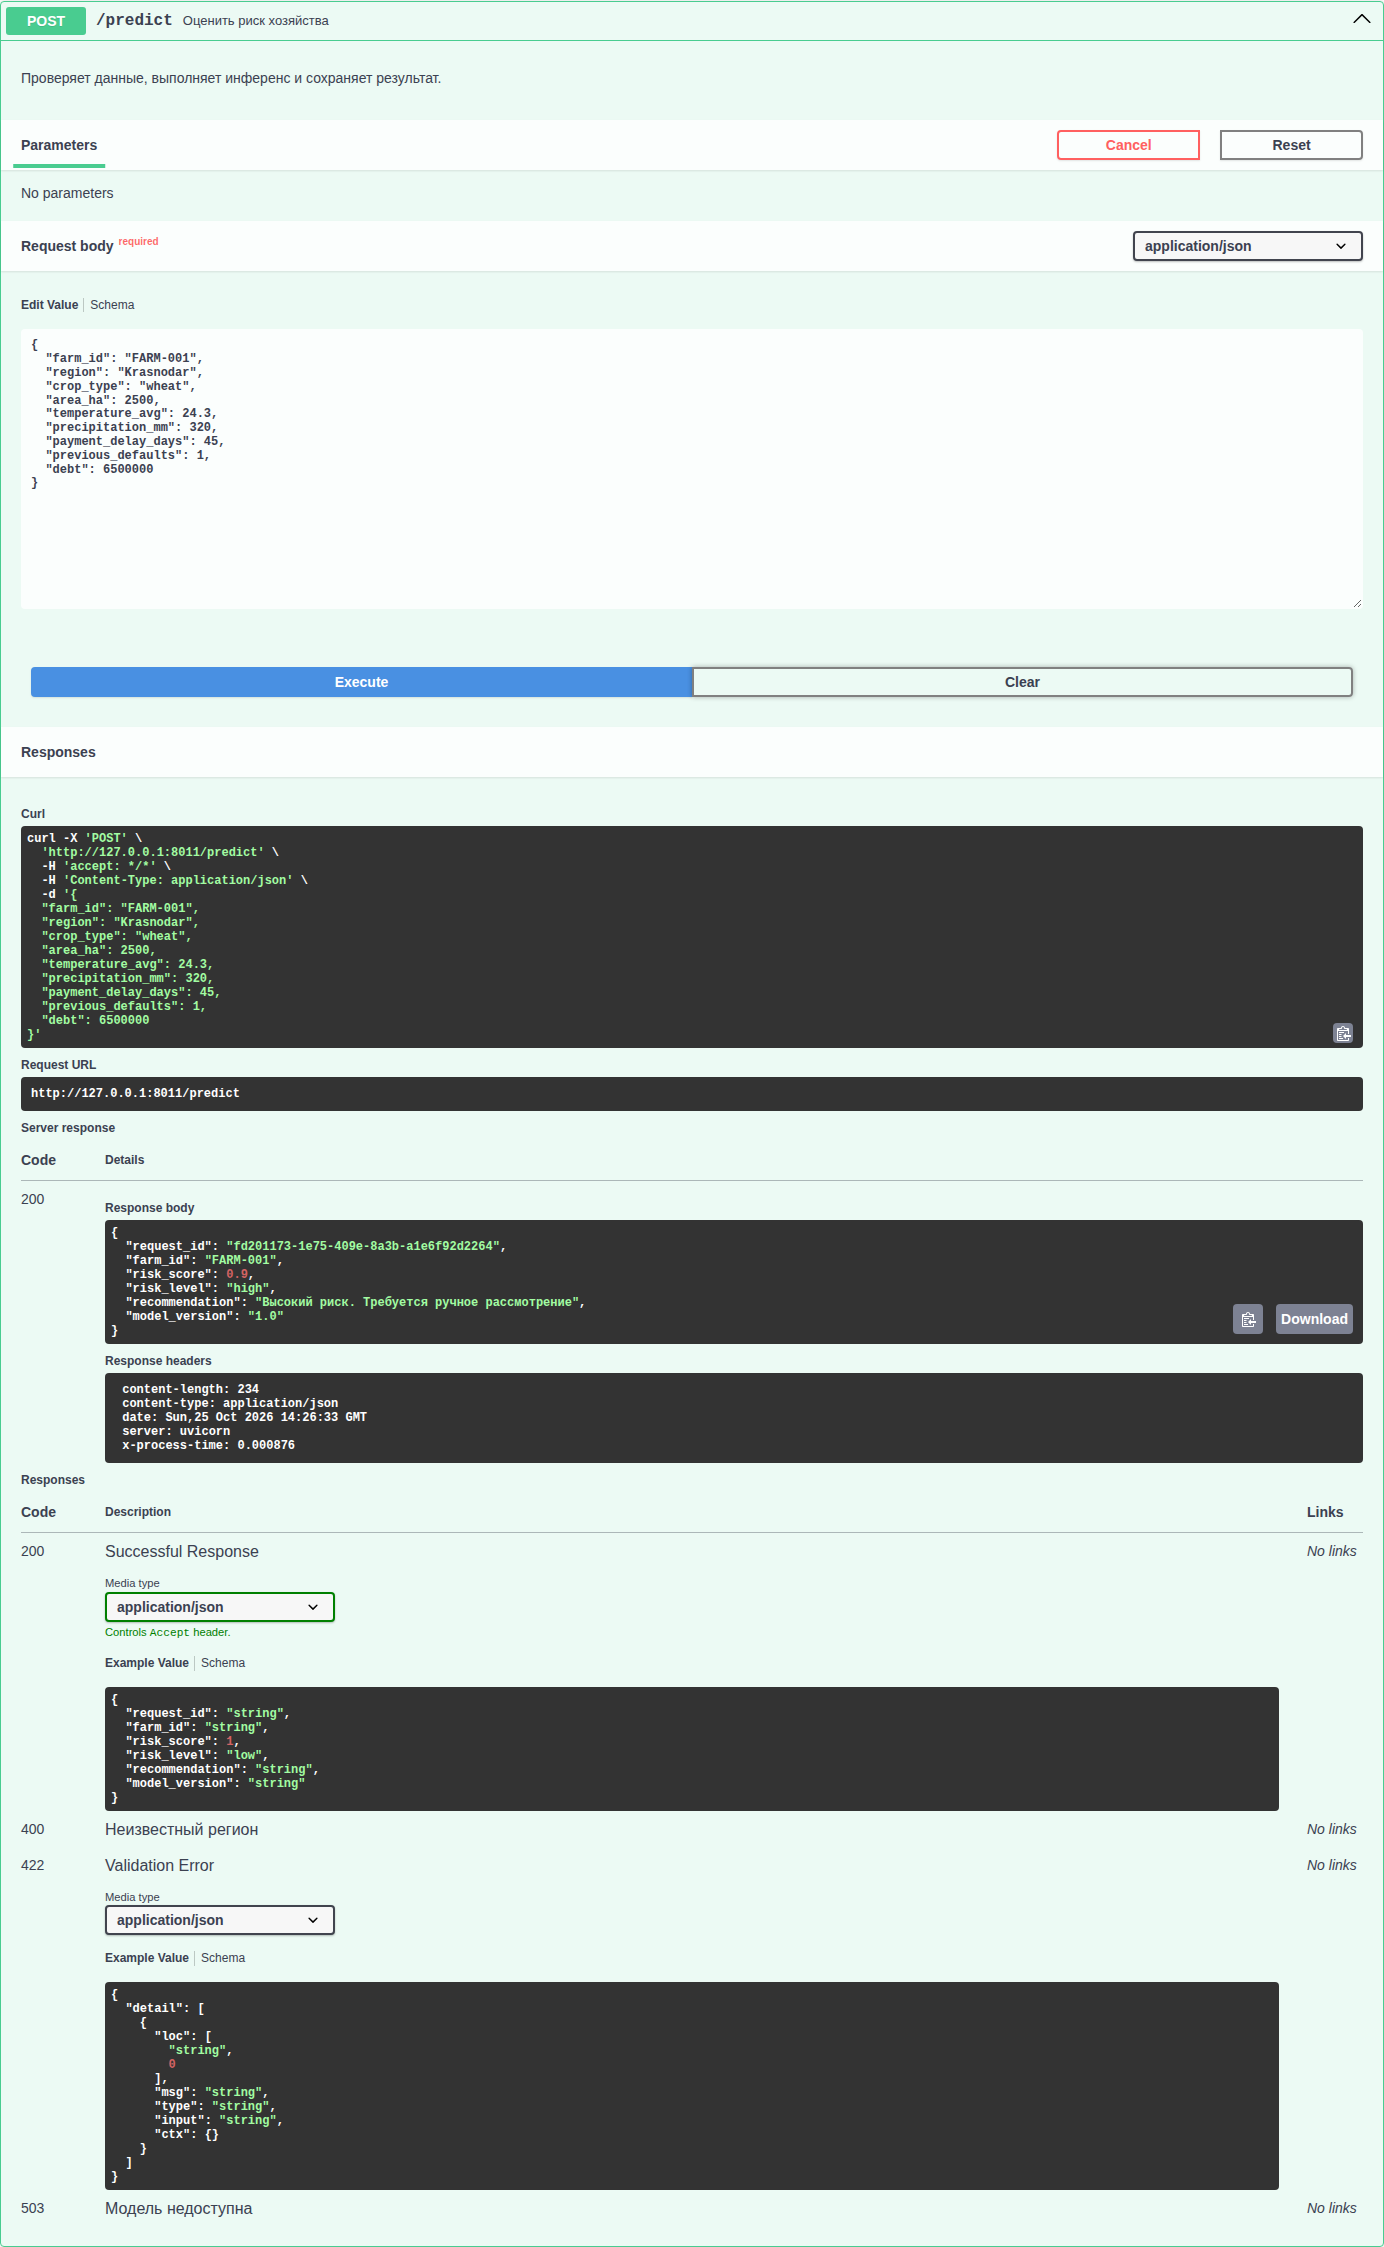
\includegraphics[width=\textwidth,height=0.78\textheight,keepaspectratio]{successful-predict.png}
  \caption{Успешный вызов POST /predict}
  \label{fig:predict-success}
\end{figure}

\subsection{Ошибка структурной валидации}

Запрос с отрицательной площадью не должен доходить до ML-модели: такое значение
нарушает контракт, делает прогноз бессмысленным и напрасно расходует
вычислительные ресурсы. FastAPI отклоняет запрос на границе сервиса со статусом
\code{422 Unprocessable Entity}.

\begin{figure}[H]
  \centering
  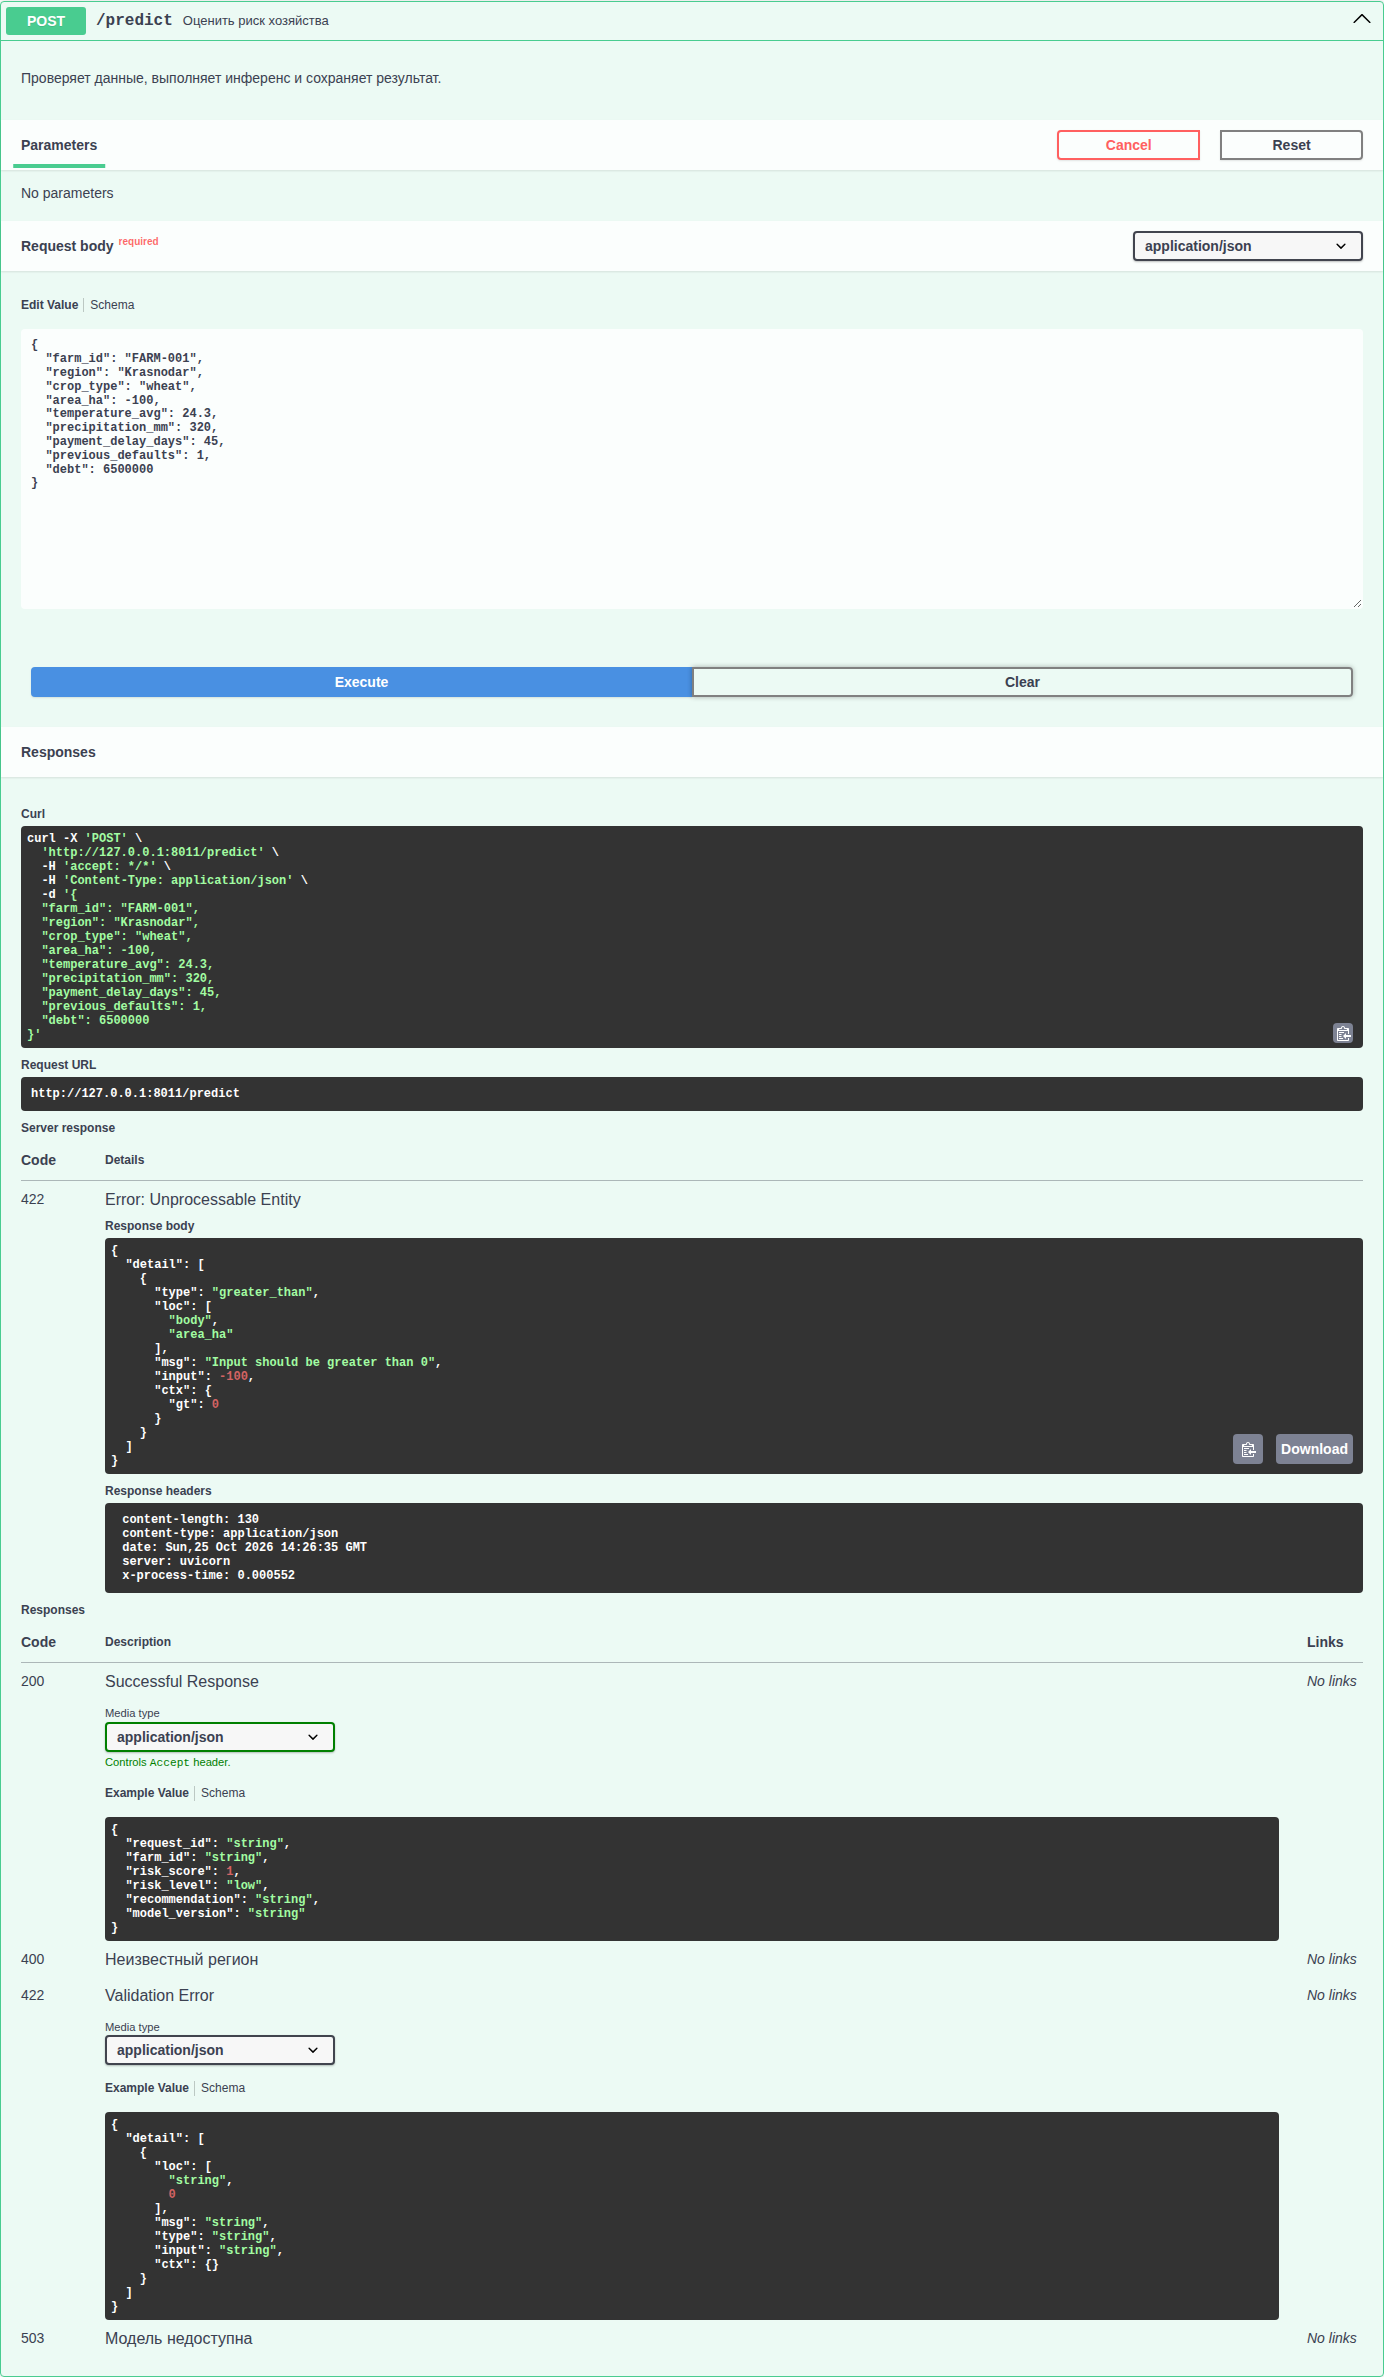
\includegraphics[width=\textwidth,height=0.78\textheight,keepaspectratio]{pydantic-error.png}
  \caption{Ошибка Pydantic при отрицательной площади посевов}
  \label{fig:pydantic-error}
\end{figure}

\subsection{Получение отсутствующего прогноза}

При обращении к неизвестному \code{request\_id} сервис возвращает статус
\code{404 Not Found} и диагностическое сообщение \code{Prediction not found}.

\begin{figure}[H]
  \centering
  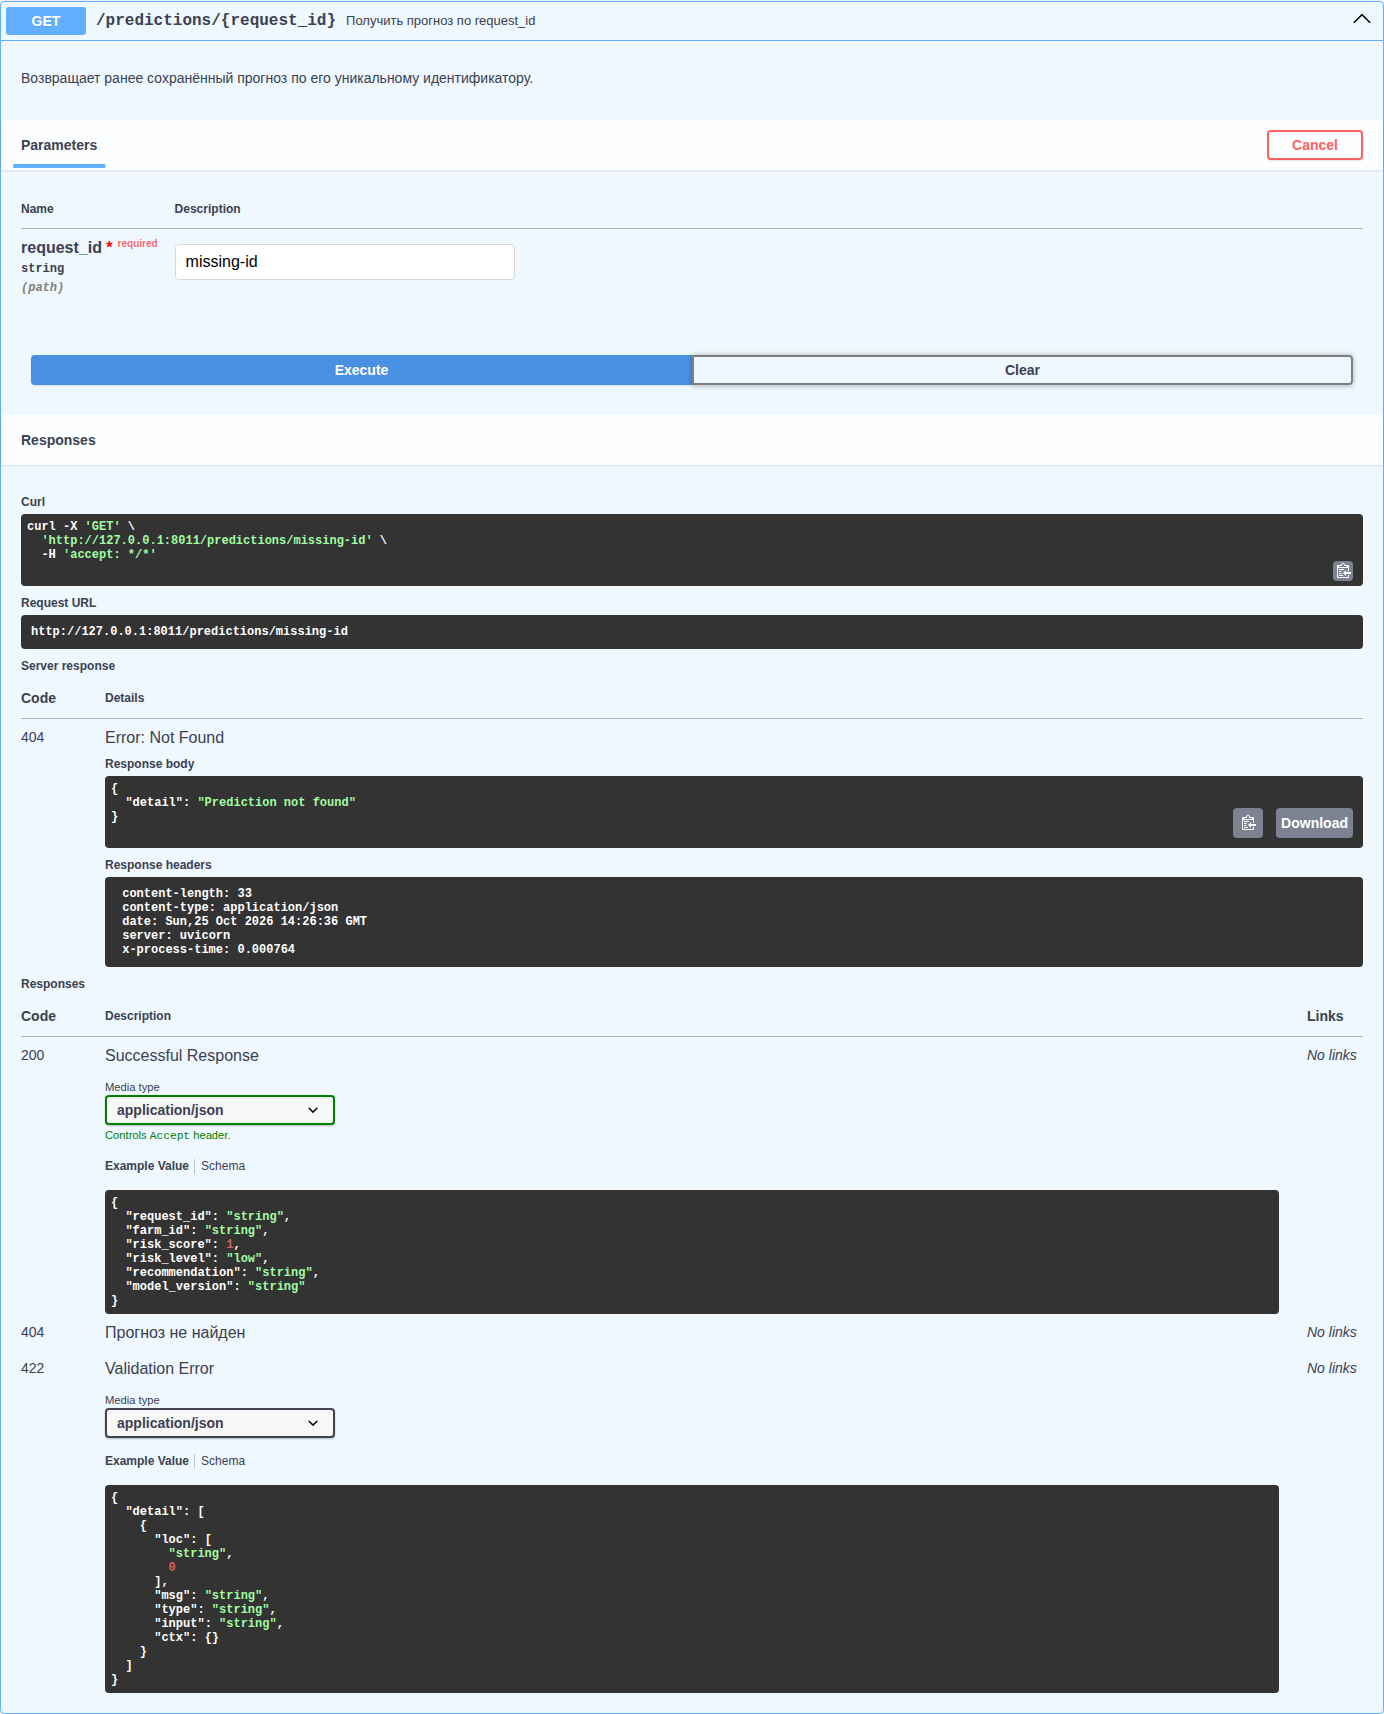
\includegraphics[width=\textwidth,height=0.78\textheight,keepaspectratio]{404-not-found.png}
  \caption{Ответ 404 для неизвестного request\_id}
  \label{fig:not-found}
\end{figure}

\section{Тестирование API}

\begin{longtable}{>{\raggedleft\arraybackslash}p{0.5cm}
                  >{\raggedright\arraybackslash}p{6.0cm}
                  >{\centering\arraybackslash}p{2.2cm}
                  >{\centering\arraybackslash}p{2.2cm}
                  >{\raggedright\arraybackslash}p{2.1cm}}
  \caption{Результаты обязательных тест-кейсов}\label{tab:tests}\\
  \toprule
  \textbf{№} & \textbf{Запрос} & \textbf{Ожидаемый код} &
  \textbf{Полученный код} & \textbf{Результат} \\
  \midrule
  \endfirsthead
  \toprule
  \textbf{№} & \textbf{Запрос} & \textbf{Ожидаемый код} &
  \textbf{Полученный код} & \textbf{Результат} \\
  \midrule
  \endhead
  \bottomrule
  \endfoot
  1 & \code{GET /health} & 200 & 200 & Пройден \\
  2 & \code{GET /model-info} & 200 & 200 & Пройден \\
  3 & Корректный \code{POST /predict} & 200 & 200 & Пройден \\
  4 & \code{area\_ha = -100} & 422 & 422 & Пройден \\
  5 & Неизвестный регион & 400 & 400 & Пройден \\
  6 & Существующий \code{request\_id} & 200 & 200 & Пройден \\
  7 & Неизвестный \code{request\_id} & 404 & 404 & Пройден \\
  8 & \code{limit = 2} & 200 & 200 & Пройден \\
  9 & \code{risk\_level = high} & 200 & 200 & Пройден \\
  10 & \code{limit = -5} & 422 & 422 & Пройден \\
\end{longtable}

Автоматические тесты дополнительно проверяют границы категорий риска,
недопустимое значение \code{risk\_level}, ответ 503 при недоступной модели,
формат UUID, наличие заголовка \code{X-Process-Time}, OpenAPI-схемы и
доступность Swagger UI. Все 20 тестов пройдены успешно.

\section{Анализ API-контракта}

\begin{longtable}{>{\ttfamily\raggedright\arraybackslash}p{3.4cm}
                  >{\centering\arraybackslash}p{1.2cm}
                  >{\raggedright\arraybackslash}p{3.0cm}
                  >{\raggedright\arraybackslash}p{3.1cm}
                  >{\centering\arraybackslash}p{1.3cm}
                  >{\raggedright\arraybackslash}p{2.5cm}}
  \caption{Анализ API-контракта}\label{tab:contract}\\
  \toprule
  \normalfont\textbf{Endpoint} & \textbf{Метод} & \textbf{Вход} &
  \textbf{Выход} & \textbf{Успех} & \textbf{Ошибки} \\
  \midrule
  \endfirsthead
  \toprule
  \normalfont\textbf{Endpoint} & \textbf{Метод} & \textbf{Вход} &
  \textbf{Выход} & \textbf{Успех} & \textbf{Ошибки} \\
  \midrule
  \endhead
  \bottomrule
  \endfoot
  /health & \normalfont GET & \normalfont --- & HealthResponse & 200 & \normalfont 500 \\
  /model-info & \normalfont GET & \normalfont --- & ModelInfoResponse & 200 & \normalfont 500 \\
  /predict & \normalfont POST & \normalfont JSON FarmRequest & PredictionResponse & 200 & \normalfont 400, 422, 503, 500 \\
  /predictions/\{request\_id\} & \normalfont GET & \normalfont path: request\_id & PredictionResponse & 200 & \normalfont 404, 500 \\
  /predictions & \normalfont GET & \normalfont query: limit, risk\_level & PredictionResponse[] & 200 & \normalfont 422, 500 \\
\end{longtable}

OpenAPI-документ явно описывает пути, HTTP-методы, обязательные поля,
ограничения и схемы ответов. Благодаря параметру \code{response\_model} внешний
контракт не зависит от внутреннего формата хранения данных.

\section{Вывод}

В ходе работы разработан модульный FastAPI-сервис агроскоринга. Сервис
валидирует входные данные, рассчитывает и сохраняет прогнозы, поддерживает поиск
и фильтрацию, возвращает семантически корректные HTTP-коды и публикует
OpenAPI-контракт.

REST API в AI-системе является стабильной границей между моделью и клиентами:
он скрывает детали реализации модели, задаёт форматы обмена и правила обработки
ошибок, а также позволяет менять внутреннюю реализацию без изменения внешних
информационных систем.

\end{document}

